
%\section{Data Overview} 





\subsection{Stripe 82 dataset} 

The equatorial stripe 82 region (22$^h$24$^m$ $<$ R.A. $<$ 04$^h$08$^m$, $-$1.27$^\circ$  $<$ $+$1.27$^\circ$, about 
290 deg$^2$) from the southern Galactic cap ($-64^\circ < b <  -20^\circ$) has been repeatedly imaged (of the order
hundered times) by SDSS to study variability phenomena (such as supernovae, asteroids, variable stars, quasar 
variability). A given observing stretch of SDSS imaging data is called a ``run''. Often there is only a single
run for a given observing run, though sometimes there are multiple runs per night. We use here seeing data for 
XXX runs, with a total of XXX fields, obtained between September, 1998 and December 2004 XXXcorrect?). All
runs are obtained during the Fall observing season (September to December). Astrometric and photometric aspects 
of this dataset have been discussed in detail by \cite{Ivezic2007} and \cite{Sesar2007}. 




\subsection{The treatment of seeing in SDSS}
 
Even in the absence of atmospheric inhomogeneities, the SDSS telescope delivers images whose 
FWHMs vary by up to 15\% from one side of a CCD to the other; the worst effects are seen in 
the chips farthest from the optical axis \citep{Gunn2006}. Moreover, since the atmospheric 
seeing varies with time, the delivered image quality is a complex two-dimensional function 
even on the scale of a single frame (for an example of the instantaneous image quality across 
the imaging camera, see Figure 7 in \citealt{SDSSEDR}). 
 
The SDSS imaging PSF is modeled 
heuristically in each band using a Karhunen-Lo\'{e}ve (K-L) transform \citep{Lupton2002}. 
Using stars brighter than roughly 20$^{th}$ magnitude, the PSF from a series of five frames is expanded 
into eigenimages and the first three terms are kept. The variation of the coefficients is fit 
with polynomials, using data from the frame in question, plus the immediately preceding and following 
half-frames. The success of this K-L expansion is gauged by comparing PSF photometry based on the 
modeled K-L PSFs with large-aperture photometry for the same (bright) stars \citep{SDSSEDR}. 
Parameters that characterize seeing for one field of imaging data are stored in the so-called psField 
files\footnote{https://data.sdss.org/datamodel/files/PHOTO\_REDUX/RERUN/RUN/objcs/CAMCOL/psField.html}. 
The status parameter flag for each frame indicates the success of the K-L decomposition.

In addition to the K-L decomposition, the SDSS processing pipeline computes parameters of the 
best-fit double Gaussian, evaluated at the center of each frame. The measured PSF profiles are 
extended to $\sim$30 arcsec using observations of bright stars and at such large radii 
double Gaussian fits underpredict the measured profiles. For this reason, the fits are extended 
to include the so-called ``power-law wings''
\begin{equation}
        PSF(r) = {\exp(-{r^2\over 2\,\sigma_1^2}) + b\,\exp(-{r^2\over 2\,\sigma_2^2})
           + p_0\left(1 + { r^2 \over \beta \sigma_P^2}\right)^{-\beta/2} \over 1 + b + p_0}.
\end{equation} 
The measured PSFs are thus modeled using 6 free parameters, and given that the measured
profiles include up to 10 data points, the fits are usually excellent. The best-fit parameters
are reported in psField files. 

 


\subsubsection{QA plots from SDSS Postage Stamp Pipeline (PSP)}

Testing (will probably be removed later): for each run, camera column and filter, PSP makes three QA plots, 
Figs.\ref{fig:PSPplot1}--\ref{fig:PSPplot3}. 


\begin{figure}
\centering
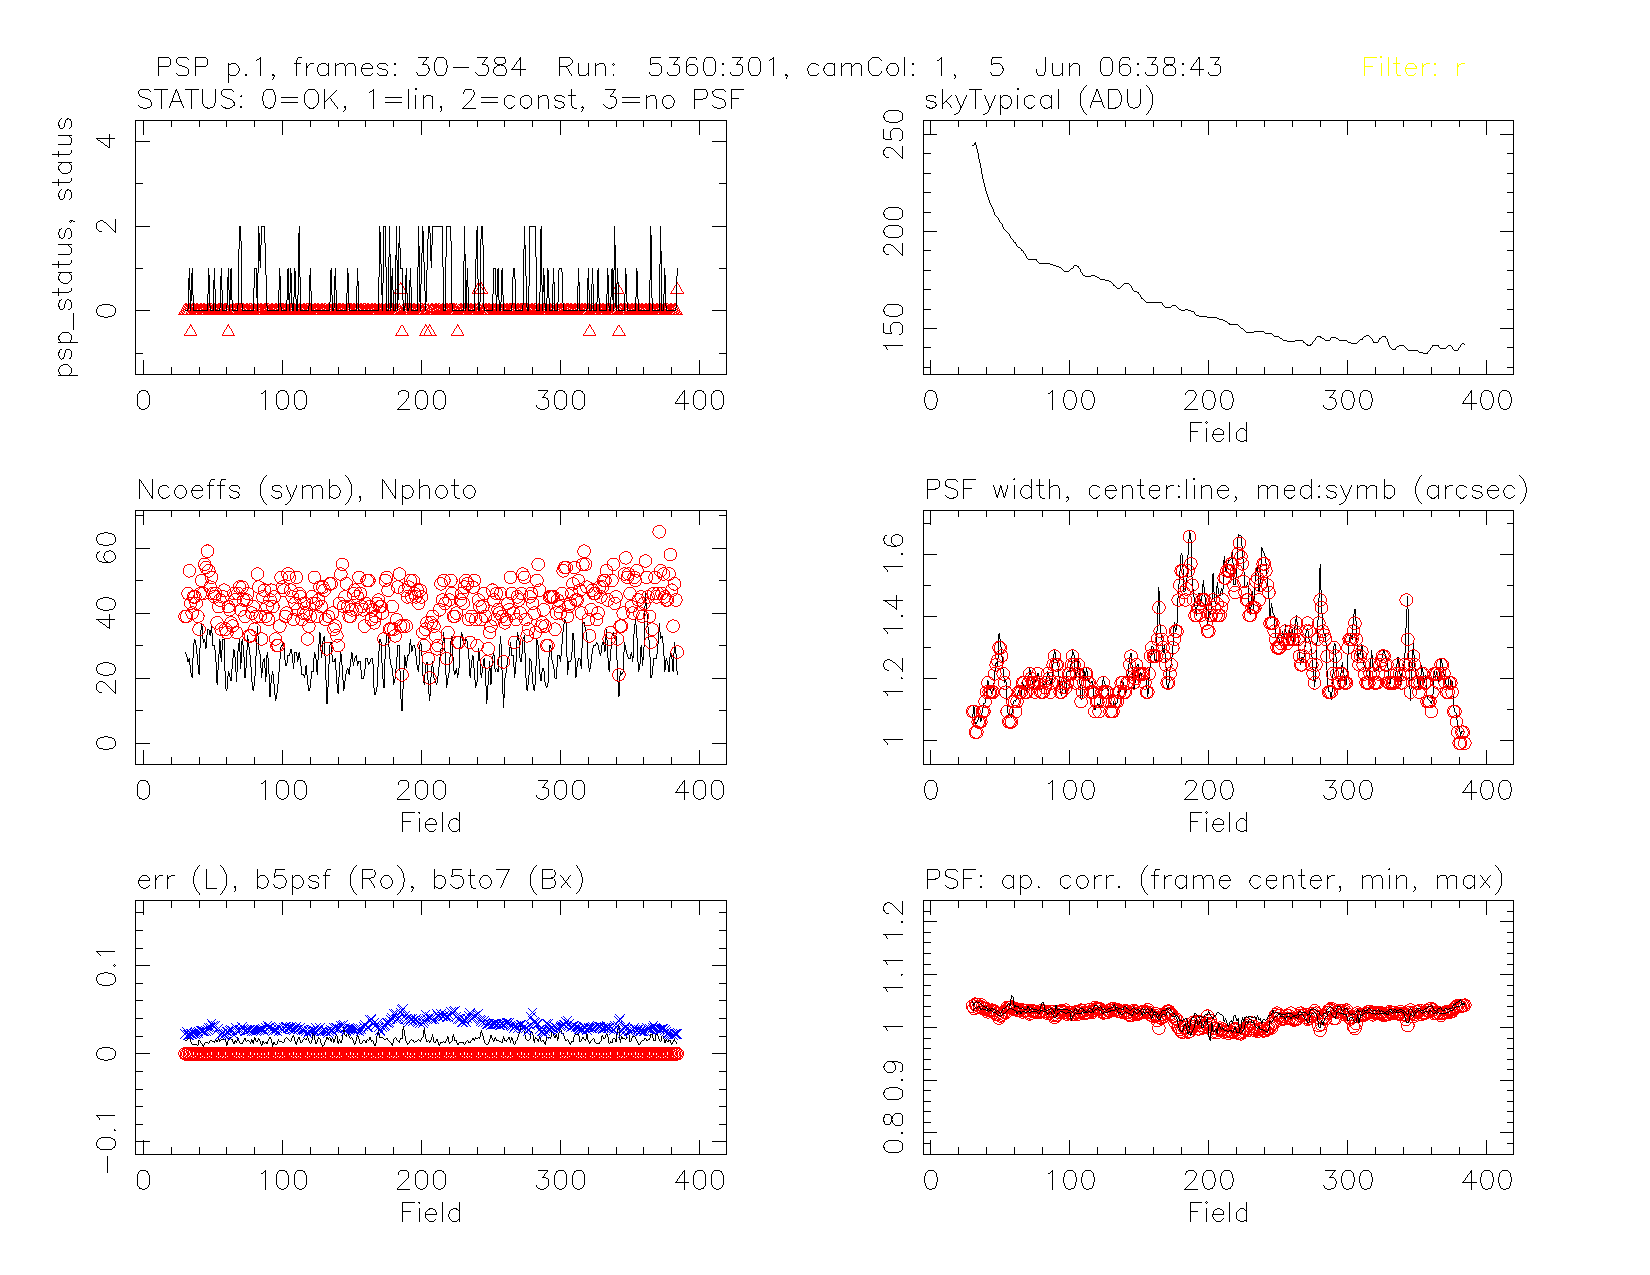
\includegraphics[width=0.9\textwidth]{FIGURES/psPlots1-005360-r1.pdf}
\caption{The plot 1 (psPlots1-005360-r1) produced by PSP for SDSS run 5306, 
camera column 1, in the $r$ band. The middle right panel shows the FWHM for
the measured seeing, as a function of field number (that is, as  function of time, 
with one field cooresponding to about 36 seconds). Note the large deterioration
of seeing between fields 130 and 300, lasting a bit under 2 hours. 
\label{fig:PSPplot1}}
\end{figure}


\begin{figure}
\centering
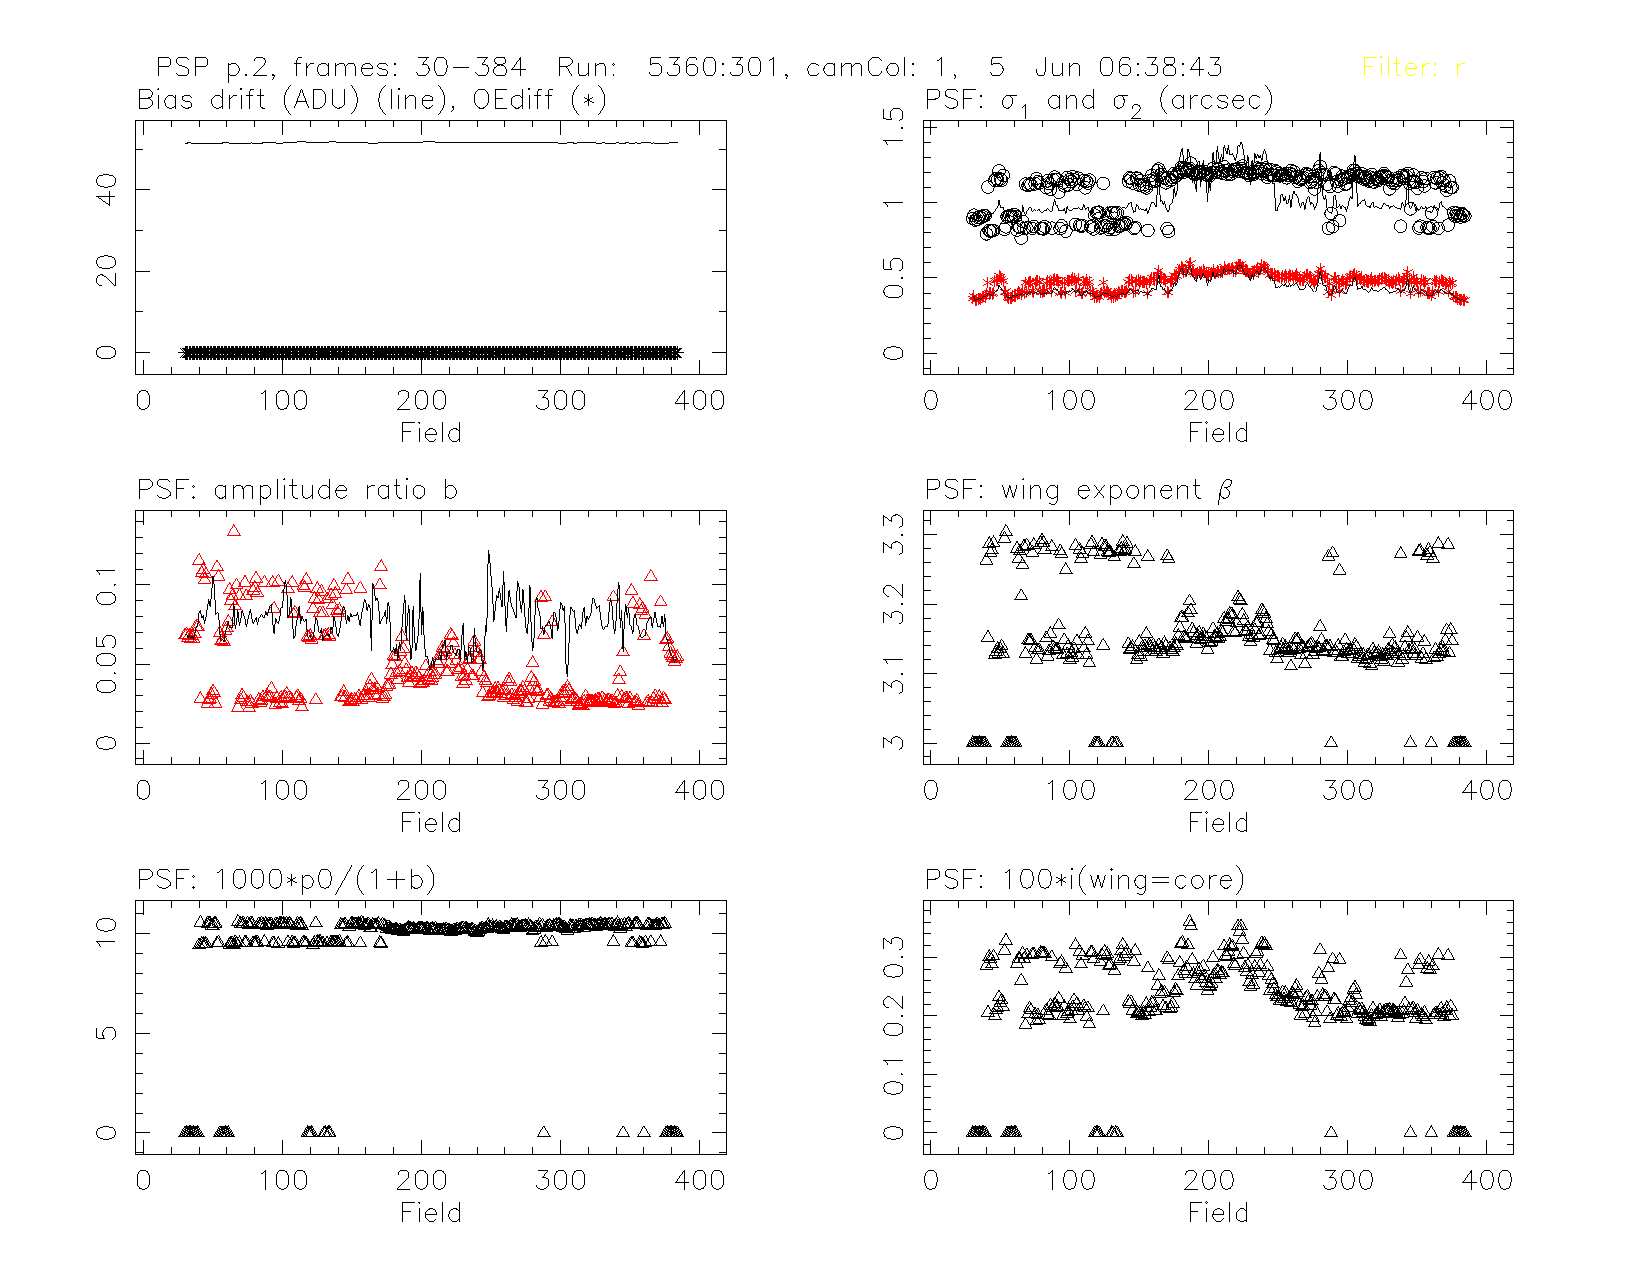
\includegraphics[width=0.9\textwidth]{FIGURES/psPlots2-005360-r1.pdf}
\caption{Similar to Fig~\ref{fig:PSPplot1}, except that here the plot 2 is shown.
Except for the top left panel, the best-fit PSF parameters (a double Gaussian
plus a power-law wing) are shown (see text for their description). 
\label{fig:PSPplot2}}
\end{figure}


\begin{figure}
\centering
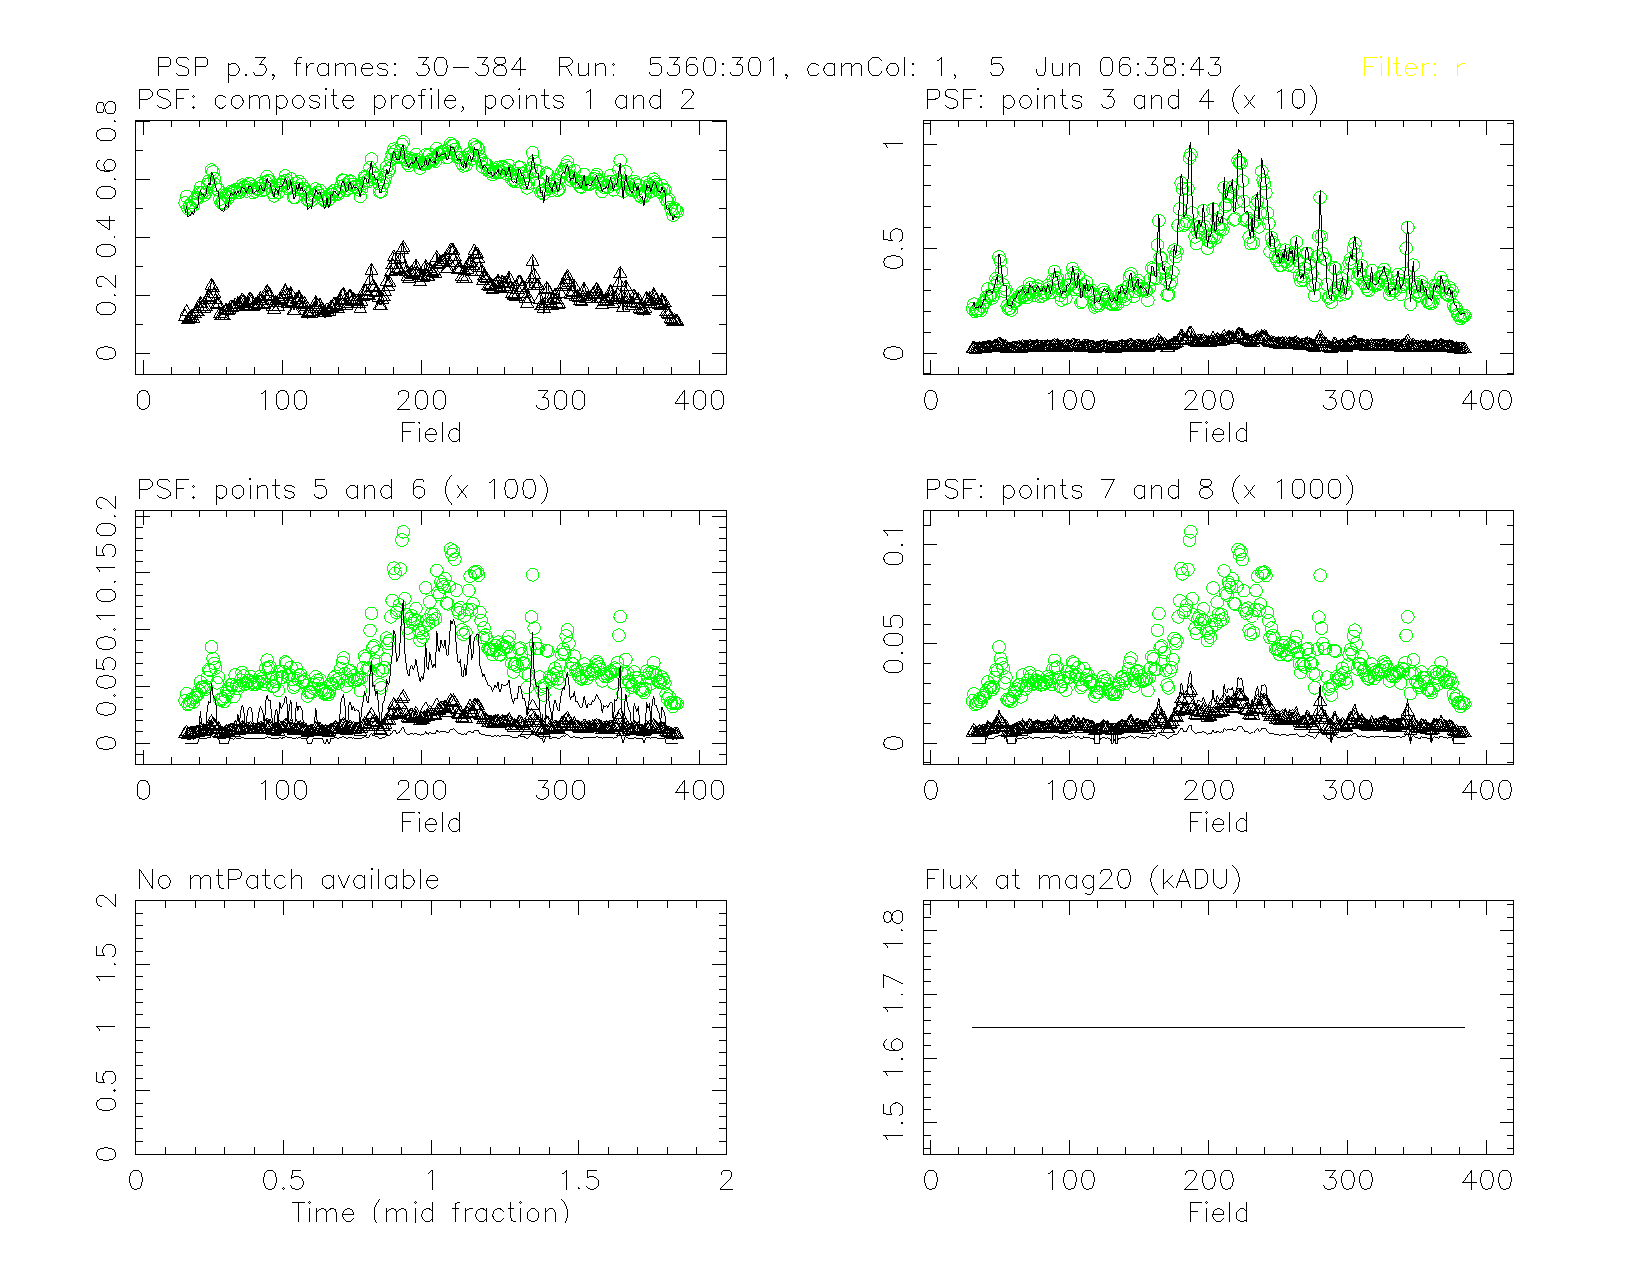
\includegraphics[width=0.9\textwidth]{FIGURES/psPlots3-005360-r1.pdf}
\caption{Similar to Fig~\ref{fig:PSPplot1}, except that here the plot 3 is shown.
The top four panels show the values of composite PSF profile (data).
\label{fig:PSPplot3}}
\end{figure}
